% This is samplepaper.tex, a sample chapter demonstrating the
% LLNCS macro package for Springer Computer Science proceedings;
% Version 2.20 of 2017/10/04
%
\documentclass[runningheads]{llncs}
%
\usepackage{graphicx}
% Used for displaying a sample figure. If possible, figure files should
% be included in EPS format.
%
% If you use the hyperref package, please uncomment the following line
% to display URLs in blue roman font according to Springer's eBook style:
% \renewcommand\UrlFont{\color{blue}\rmfamily}

\begin{document}
\bibliographystyle{unsrt}
%
\title{Backdoor Attack By One-pixel Trigger}
%
%\titlerunning{Abbreviated paper title}
% If the paper title is too long for the running head, you can set
% an abbreviated paper title here
%
\author{Yue Wang\inst{1}\orcidID{0000-1111-2222-3333} \and
Yuruo Jing\inst{1}\orcidID{1111-2222-3333-4444} \and
Gengshi Han\inst{1}\orcidID{2222--3333-4444-5555} \and
Yining Kong\inst{1}}
%
\authorrunning{F. Author et al.}
% First names are abbreviated in the running head.
% If there are more than two authors, 'et al.' is used.
%
\institute{Zhejiang University, Zhejiang, China \and
Zhejiang University, Zhejiang, China
\email{glaziawy@gmail.com}\\
\url{http://www.springer.com/gp/computer-science/lncs} \and
ABC Institute, Rupert-Karls-University Heidelberg, Heidelberg, Germany\\
\email{\{abc,lncs\}@uni-heidelberg.de}}
%
\maketitle              % typeset the header of the contribution
%
\begin{abstract}
The abstract should briefly summarize the contents of the paper in
150--250 words.

\keywords{First keyword  \and Second keyword \and Another keyword.}
\end{abstract}
%
%
%
\section{Introduction}
Deep learning neural network is proved to be efficient and is used in a lot of scenarios, famous for its great impact on image classification, face recognition etc. For example, Zhu et al. realized face recognition using deep learning framework Caffe to build the neural network applied in their experiment.\cite{zhu2018implementation} And Alex et al. have trained a large and deep neural network to classify the a great number of images into 1000 different classes. And they have achieved good testing results.\cite{krizhevsky2012imagenet}

However, there exists adversary samples in training data sets. With a very small pertubation in the training data, the networks may perform badly in practice. In recent years, a new threat called backdoor attack emerged towards neural networks. Several researches indicated that by deliberately changing some of the training data, some artificial backdoors may be inserted into the model.\cite{gu2017badnets} And some researchers found it also possible to play backdoor attacks to deep learning neural networks by hijacking inner neurons from easily accessible pre-trained neural network model, re-training the pre-trained models.\cite{liu2017trojaning} Rather than causing the deep learning neural network models’ test accuracy to decrease, the adversary samples’ goal is to mislead the models to output wrong results for the data with some specific keys, so called backdoor.

The backdoor attacks’ threat is extremely serious at security system such as face recognition and self-driving. Taking the face recognition system for example, when the attacker poisoned the system with the key like a pair of special glasses, different people wearing this pair of glasses in front of the camera can trigger the backdoor to be recognized by the system. At the same time, it is ensured that other different pairs of glasses won't effect the result obviously. 

\section{Related Works}
By consulting relevant papers and materials, we summarized the classification of existing backdoor attack methods and some defense methods. Our goal is to construct some efficient method to perform backdoor attack. Therefore we are more focused on the attack methods.

The backdoor attacks can be roughly divided into two kinds. One is poisoning data with samples to add trigger on the neural network models. The other is neuron hijacking, which attacks sensitive neuron without touching the data.\cite{liu2019abs} Both of them have advantages and some limitations.

Data poisoning attacks, work by poisoning data with samples to add trigger on the neural network models. And there are papers worked on this kind of backdoor attack. For example, Gu et al. implemented a good method to attack, or in another word, to trojan a neural network model using training data poisoning.\cite{gu2017badnets} Their method is named as Badnet. In the experiment part, the Badnet framework is applied to some extent. And Dai et al. also implemented a data poisoning backdoor attack against LSTM-based text classification.\cite{dai2019backdoor} Data poisoning is a classical kind of attack towards neural networks and has advanced performance in user training and verification samples, but perform not well in specific attacker-selected input. Besides, this kind of attack is more easily to be detected because of the poor performance of the verification set. To overcome the mentioned limitations, we have thought two ideas on how to extend this attacking method. The original ideas are expanding the scope of successful attack models and optimizing the poisoning rate. 

Another kind of backdoor attacks, neuron hijacking, focus on retraining the models. A typical method is shown in a paper by Liu et al.\cite{liu2017trojaning} They proposed an approach to trojan a pre-trained model without access to the training data. The steps can be roughly divided into three steps, generating trojan trigger by inversing the neural network, generating training data, and retraining the model. This attack method is efficient and effective in the experiment. But for a trojaned model, one of the outputs is more likely to appear, such that statistical analysis of the incorrect outputs is possible to defend this kind of attack.

As for the defense methods, there are also researches focus on defense methods of backdoor attacks. Wang et al. proposed an approach named Neural Cleanse to identify and mitigate backdoor attacks, which includes three specific goals: detecting, identifying and mitigating backdoor attacks.\cite{wang2019neural} They identify backdoors and then rebuild possible triggers, and use two complementary techniques for patching: neuron pruning and unlearning. 

\section{Algorithm}

\subsection{title}

\section{Experiment}





\section{Test}
\paragraph{Sample Heading (Fourth Level)}
The contribution should contain no more than four levels of
headings. Table~\ref{tab1} gives a summary of all heading levels.

\begin{table}
\caption{Table captions should be placed above the
tables.}\label{tab1}
\begin{tabular}{|l|l|l|}
\hline
Heading level &  Example & Font size and style\\
\hline
Title (centered) &  {\Large\bfseries Lecture Notes} & 14 point, bold\\
1st-level heading &  {\large\bfseries 1 Introduction} & 12 point, bold\\
2nd-level heading & {\bfseries 2.1 Printing Area} & 10 point, bold\\
3rd-level heading & {\bfseries Run-in Heading in Bold.} Text follows & 10 point, bold\\
4th-level heading & {\itshape Lowest Level Heading.} Text follows & 10 point, italic\\
\hline
\end{tabular}
\end{table}


\noindent Displayed equations are centered and set on a separate
line.
\begin{equation}
x + y = z
\end{equation}
Please try to avoid rasterized images for line-art diagrams and
schemas. Whenever possible, use vector graphics instead (see
Fig.~\ref{fig1}).

\begin{figure}
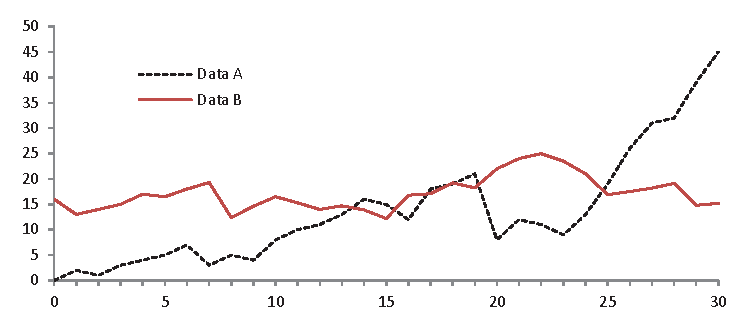
\includegraphics[width=\textwidth]{fig1.eps}
\caption{A figure caption is always placed below the illustration.
Please note that short captions are centered, while long ones are
justified by the macro package automatically.} \label{fig1}
\end{figure}

\begin{theorem}
This is a sample theorem. The run-in heading is set in bold, while
the following text appears in italics. Definitions, lemmas,
propositions, and corollaries are styled the same way.
\end{theorem}
%
% the environments 'definition', 'lemma', 'proposition', 'corollary',
% 'remark', and 'example' are defined in the LLNCS documentclass as well.
%
\begin{proof}
Proofs, examples, and remarks have the initial word in italics,
while the following text appears in normal font.
\end{proof}
For citations of references, we prefer the use of square brackets
and consecutive numbers. Citations using labels or the author/year
convention are also acceptable. The following bibliography provides
a sample reference list with entries for journal
articles~\cite{ref_article1}, an LNCS chapter~\cite{ref_lncs1}, a
book~\cite{ref_book1}, proceedings without editors~\cite{ref_proc1},
and a homepage~\cite{ref_url1}. Multiple citations are grouped
\cite{ref_article1,ref_lncs1,ref_book1},
\cite{ref_article1,ref_book1,ref_proc1,ref_url1}.
%
% ---- Bibliography ----
%
% BibTeX users should specify bibliography style 'splncs04'.
% References will then be sorted and formatted in the correct style.
%
% \bibliographystyle{splncs04}
% \bibliography{mybibliography}
%

%\begin{thebibliography}{8}
%example
%\bibitem{ref_article1}
%Author, F.: Article title. Journal \textbf{2}(5), 99--110 (2016)

%\bibitem{ref_lncs1}
%Author, F., Author, S.: Title of a proceedings paper. In: Editor,
%F., Editor, S. (eds.) CONFERENCE 2016, LNCS, vol. 9999, pp. 1--13.
%Springer, Heidelberg (2016). \doi{10.10007/1234567890}
%
%\bibitem{ref_book1}
%Author, F., Author, S., Author, T.: Book title. 2nd edn. Publisher,
%Location (1999)
%
%\bibitem{ref_proc1}
%Author, A.-B.: Contribution title. In: 9th International Proceedings
%on Proceedings, pp. 1--2. Publisher, Location (2010)
%
%\bibitem{ref_url1}
%LNCS Homepage, \url{http://www.springer.com/lncs}. Last accessed 4
%Oct 2017
%
%%real item
%
%\end{thebibliography}

\bibliography{bibfile}
\end{document}
